\section{Light curves}

The main concept present on the photometric analysis of variable stars is the light curve:
a diagram representing the \textbf{temporal} evolution of the star's \textbf{brightness}. 
Light curves are used to describe all types of variable stars, both periodic and non-periodic. 
In the case of periodic variable stars, a \textbf{phased} light curve is often preferred.

In order to properly study variable star, we need to have solid definitions for \enquote{temporal}, 
\enquote{brightness} and \enquote{phase} measurements.

\subsection{Julian Dates}
	
	\intent{Common calendars as a mixed-radix complicated unit}
	
	Calendars have existed for as long as humans have been able to keep track of time; since the dawn of astronomy.
	But similarly to the astronomical and physical sciences, calendars change with culture and also with time itself.
	The daylight, lunar and seasonal cycles do not align nicely; their periods are not a simple fraction of each others.
	This causes all calendars that try to align the day period with any other solar system based period to be a mixed radix unit full of exceptions.
	If your calendar is moon-based, your months will have unequal number of days.
	If your calendar is season-based, your years will have unequal number of days.
	Either way, computing day differences will be a nightmare. 
	You cannot have an integer calendar without leap days every few years.
	
	\intent{Troubled days}
	
	So, the only option is to do neither and just count the number of days. 
	But as discussed before, the year to day ratio is far from a simple fraction;
	by the time the earth makes a full revolution around the sun (with respect to the other stars),	a non-integer number of days have passed.
	But this seems fine, then. If you accept to deal with decimals, you can just take your base unit as a solar day, noon to noon,
	easy enough to measure and compare.
	
	\intent{Atomic clocks confidence}
	
	Except, the solar day is not exactly constant. The time from terrestrial noon to noon is not a constant number of seconds \citep{McCarthy1986}.
	Now what, measure everything in seconds? will the same argument hold here, and the second will turn out to be variable? 
	It turns out we have a very constant, precise definition for a second. 
	According to the 2019 redefinition of the International System of Units (SI),
	one second is exactly \citep{si-brochure}:
	\begin{equation}
		1\text{ s} = \frac{9\,192\,631\,770}{\Delta\nu_{\text{Cs}}} \label{eq:SI-second}
	\end{equation}
	Where $\Delta\nu_{Cs}$ is the unperturbed ground-state hyperfine transition frequency of ${}^{133}\text{Cs}$, which is a fundamental physical constant.
	Then, supported by hundreds of years of experiments in the natural sciences, we measure everything in seconds. 
	
	\intent{The Unix Time and the Julian Date}
	
	%A commonly used time unit based on this definition is the (TAI-based) Unix Time: 
	%the number of seconds since January 1st 1970, without leaps \citep[XRAT A.4.16]{POSIX2017}.	
	But for astronomical events, seconds are a tiny unit. Measuring temporal scales of days and years in seconds is cumbersome and unpopular.
	Besides, historical astronomical records ---even Before the Common Era--- were and are still in use \citep{Morrison2004},
	and astronomers and historians liked to have a unit of time that did not extend to the negative numbers.
	Therefore astronomical dates were historically to be measured in days since a date early enough to capture historical records.
	The original idea for this zero point came from Joseph Scaliger in 1583 \citep{Carroll2017}. 
	He considered three time periods used in his day:
	
	\begin{itemize}
		\item The solar cycle: in the Julian calendar, the weekday of a given date on the year would repeat every 28 years 
			\footnote{With exactly $365.25 = 1461/4$ days in a year and 7 days a week, the week days cycle every $\text{LCM}(1461,7)=10227$ days, $=28$ years.}. 
			The solar number of a (Julian) calendar year $y$ in this cycle is given by
			\begin{equation}
				\text{SolarNumber}(y) = \text{mod}(y+8,28) + 1
			\end{equation}
			
		\item The lunar cycle: 19 years, the number of years in which a moon phase will occur in the same day of the year
			\footnote{A mean synodic month (time between two full moons) is 29.53059 days. 235 synodic months was sufficiently close to 19 years for the Julian calendar.}.
			The so called \enquote{Golden Number} of a Julian year $y$ is given by 
			\begin{equation}
				\text{GoldenNumber}(y) = \text{mod}(y,19)+ 1
			\end{equation}
			
		\item the Indiction: a 15 year period for tax census used by the Roman Empire and later by the Holy Roman Empire. Its calculation for a Julian year is:
			\begin{equation}
				\text{Indiction}(y) = \text{mod}(y+2,15) + 1
			\end{equation}
	\end{itemize}
	
	The phases on the modulus operations are selected such that historical records make sense. The solution, then to the integer equation 
	\begin{equation}
		\text{SolarNumber}(y) = \text{GoldenNumber}(y) = \text{Indiction}(y) = 1
	\end{equation}
	is, using the Chinese remainder theorem,
	\begin{equation}
		y = 3268 + 7980 n
	\end{equation}
	were $n$ is any whole number. Scaliger selected $n=-1$ as the zero point for the Julian Day system, which would be Julian year $-4712$ CE, 
	and as there was no year 0, that would be Julian $4713$ BCE, or in the Gregorian modern calendar, noon of November 24, 4714 BCE (Epoch).
	
	\intent{Final definition and the R\o{}mer Delay}
	
	Those are the ingredients needed to define the modern Julian Day system. If an Ephemeris Day is defined as $24\times60\times60=86400$ SI seconds, 
	the Julian Day (JD) is the fractional number of Ephemeris days that have passed since noon of November 24, 4714 BCE on the current calendar. 
	There are at least 4 principal corrections to the Julian Day due to astronomical, geological or relativistic effects \citep{Eastman2010}, 
	but here we will only consider one of them, as it's the only strictly needed to understand the data used on this work.
	As earth moves around the sun, the light from a distant object may reach its surface with different time delays, consequence of the finite speed of light.
	In order to be able to accurately compare time series taken around all positions of earths orbit, 
	the signal is corrected with a delay as if the measurement was taken on the position of the sun.
	This is called \textbf{Heliocentric Julian Day} (HJD), and that correction is given by (see \autoref{fig:romer-delay}):
	\begin{equation}
		\Delta t = \frac{\vec{r}\cdot \hat{n}}{c} = - \frac{r}{c} \left(\cos\delta \cos \delta_{\odot}\cos(\alpha-\alpha_\odot)+ \sin\delta \sin \delta_\odot\right)
	\end{equation}
	where $\vec{r}$ is the vector sun-to-earth, $\hat{n}$ is the direction of the measurement on earth's sky, 
	and $(\alpha,\delta),\,(\alpha_\odot,\delta_\odot)$ are the equatorial coordinates of the observed object and the sun respectively, 
	as seen from earth, \textit{i.e.} $\vec{r} = (r,\phi=\frac\pi2-\delta_\odot,\theta=\alpha_\odot)$, $\hat n = (1,\phi=\frac\pi2-\delta,\alpha)$ 
	The maximum possible value for this correction is $\sim 1 \text{ AU}/c = 16.63 \text{ min } = 0.00577$ Ephemeris days.
	
	
	
	
	\subsubsection{Remark about floating point representations}
	
	\intent{Unit in last place of floating point data}
	
	Typically, decimal numbers are stored on a computer as a double-precision floating point number, 
	which is basically \enquote{fixed point} scientific notation in base 2, with 52 binary digits for the mantissa and 11 for the exponent \citep{IEEE2019}.
	Floating point numbers are of course imprecise, and in fact more as the number they represent grows. 
	To quantify this loss of precision exists the notion of the machine epsilon: 
	the difference from a given number to the next representable number on the system.
	This epsilon (also called \enquote{unit in last place}) is greater for greater numbers,
	and there is the question of whether we will lose or not our anhelated temporal scale precision.
	
	\intent{typical precision of the numbers used}
	
	As a random example from the OGLE IV database (see \autoref{sec:data}), let's check the precision at $\text{HJD}=2455262.5065$. 
	In \autoref{lst:c-eps} there is a simple function to estimate the precision. 
	If we use it with our number we'll get $\sim 4.6\times 10^{-10}$ days, which is $40 \,\mu \text{s}$. 
	If instead of the HJD we choose to store the number of seconds since the Julian Epoch ($\sim 2.12\times 10^{11} \,\text{s}$) 
	the precision would be $\sim 30 \,\mu \text{s}$.
	But this HJD in particular was stored as a \textit{reduced} HJD. In this case, the reported number was $\text{RHJD}=\text{HJD}-2.45\times 10^6 = 5262.5065$.
	The machine precision at $5262.5065$ is $\sim 9.09\times 10^{-13} $ days, or $78.5 \,\text{ns}$, 
	so we conclude that floating point precision is not a problem for the storage of this reduced time unit in this case.
	
\subsection{Magnitudes}

	\begin{figure}[H]
		\centering
		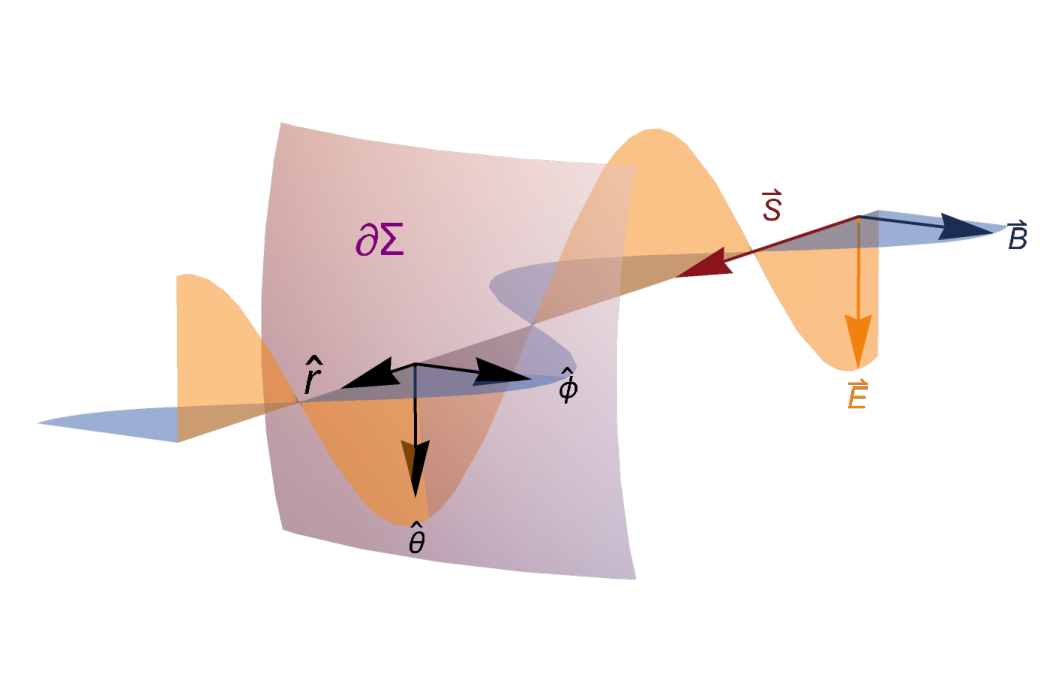
\includegraphics[width=0.6\textwidth]{img/Spherical_EM.pdf}
		\caption[Electromagnetic wave propagation through a spherical surface]{
			An electromagnetic wave ($\vec E,\vec B$) propagating outwards ($\vec S$) through a spherical surface $\partial \Sigma$ in a vacuum space.
			The correspondence of the directions of $\vec S,\vec B$ and $\vec E$ with the spherical directions $\hat r,\hat \phi, \hat \theta$ is to be noted.
		}
		\label{fig:spherical-em}
	\end{figure}
	
	\subsubsection{Energy conservation and the inverse square law}

	The magnitude system, vertical axis of a light curve, can be understood from the principles of electromagnetic waves.
	We would first want to ascertain the distance dependence of the energy flux for an isotropic light source.
	Here, isotropic means that the magnitude of the electric and magnetic fields of the wave would not depend on any angle.
	In spherical coordinates, for an outgoing wave of frequency $\omega$ and wave number $k$, we have (see \autoref{fig:spherical-em})
	\begin{equation}
		\vec E = E(r) \cos(kr-\omega t) \hat\theta \qquad \vec B = B(r) \cos(kr-\omega t) \hat\phi
	\end{equation}
	where $B(r)=E(r)/c$. Using Poynting's theorem \citep[\S8.1.2]{Griffiths2013} we can calculate the total energy flux\footnote{All the \enquote{energy fluxes} referred in this section are per unit of time.} through an entire sphere centered at the source.
	Fist, we calculate the Poynting vector 
	\begin{equation}
		\vec S = \frac{\vec E \times \vec B}{\mu_0} = \frac{\cos^2(kr-\omega t)E(r)^2}{c\mu_0} \,\hat r
	\end{equation}
	and its temporal mean 
	\begin{equation}
		\left<\vec S \right> = \frac{\omega}{2\pi}\int_0^{2\pi/\omega} \frac{\cos^2(kr-\omega t)E(r)^2}{c\mu_0} \,\hat r\;dt = \frac{E(r)^2}{2c\mu_0}\,\hat r \label{eq:poynting}
	\end{equation}

	Its flux is then the energy density flux through the whole spherical surface $\Sigma$ of radius $r$, also called Luminosity
	\begin{equation}
		L = \oint_{\partial\Sigma} \left<\vec S\right> \cdot d\vec{A} 
			= \oint_{\partial\Sigma} \left<\vec S\right> \cdot \hat r \; r^2 d\Omega
			= \oint_{\partial\Sigma} \frac{E(r)^2 r^2}{2c\mu_0} d\Omega
			= \frac{2\pi r^2  E(r)^2}{c\mu_0} \label{eq:luminosity}
	\end{equation}

	But the luminosity should \textit{not} be a function of the radius. 
	The electromagnetic energy that passes through a $r_0$-radius sphere should be the same that later passes through a $2r_0$-radius sphere.
	It's the same electromagnetic wave after all; there are no charges or currents. 
	Therefore, the magnitude of the electric field $E(r)$ should be inversely proportional to $r$, and that way $L$ is constant and energy is conserved.
	
	Knowing $E(r)$ we can then do the same process the other way around: 
	calculate the energy flux through a properly aligned detector of known area $A$,
	simply known as Flux	
	\begin{equation}
		F = \int_{S} \left<\vec S\right> \cdot \hat r \; dA = \frac{E(r)^2 A}{2 c \mu_0}
	\end{equation}
	where the integration occurs along the surface $S$ of the detector, which typically would be flat surface, 
	but considered here as a section of a sphere with a radius so immense that the difference is meaningless.
	As $E(r)\propto 1/r$, $F\propto 1/r^2$,  or equivalently, 
	\begin{equation}
		F(r)=\frac{L A}{4\pi r^2} \label{eq:flux}
	\end{equation}
	
	\subsubsection{Logarithmic scales}
	
	Working with the same example as before, if we put our detector at a distance $r=r_0$ of a source of light $a$,
	and measure a flux $F_a(r_0)$,
	the flux at a distance $2r_0$ will be $F_a(r_0)/4$, according to \autoref{eq:flux}. 
	In general, if we change the distance by a factor $d$, the change in flux would be $1/d^2$.
	
	But what if we wanted a brightness scale where \textit{multiplicative} changes on the distance became \textit{additive} changes of brightness?
	If we are confident in our measurement of $F_a(r_0)$, we could measure the fluxes relative to $F_a(r_0)$, 
	and define a new logarithmic unit for the brightness of any object $b$ as
	\begin{equation}
		\mathcal{F}_b(r) = \alpha \ln\left(\frac{F_b(r)}{F_a(r_0)}\right) \label{eq:general-magnitude}
	\end{equation}
	where $\alpha$ is a free parameter of our unit system. 
	That way, the \enquote{brightness} difference between a measure of object $b$ at distances $r_1$ and $r_2$ would be
	\begin{equation}
		\Delta \mathcal{F}_b = \mathcal{F}_b(r_2) - \mathcal{F}_b(r_1) 
			= \alpha \ln\left(\frac{F_b(r_2)}{F_b(r_1)}\right)
			= -2\alpha \ln\left(\frac{r_2}{r_1}\right)
			\label{eq:general-distance-modulus}
	\end{equation}
	where we used \autoref{eq:flux} as before. 
	One immediate consequence of this definition of brightness is that the brightness of the reference object $a$ at distance $r_0$ would be exactly 0.
	
	For our $\mathcal{F}$ to become the standard magnitude system, we have to choose $\alpha$, and $F_a(r_0)$
	
	\subsubsection{Historical choice for $\alpha$}
	
	In order to formalize the magnitude scale, and still maintain some sense with the historical records, 
	\cite{Pogson1856} proposed that an increment of 5 magnitudes would correspond to a flux 100 times \textit{smaller}. 
	That means that a magnitude 5 object would have a flux $F_b = F_a(r_0)/100$. 
	Replacing that in \autoref{eq:general-magnitude} and solving for $\alpha$ results in
	$$
		5 = \alpha \ln\frac{1}{100} \qquad \Rightarrow \qquad \alpha = \alpha = -\frac{5}{\ln 100} = -\frac{5}{\log_{10}(100)\ln(10)} = -\frac{2.5}{\ln 10}
	$$
	which allows us to rewrite \autoref{eq:general-magnitude} as 
	\begin{equation}
		\mathcal{M}_b(r) = -2.5 \log_{10}\left(\frac{F_b(r)}{F_a(r_0)}\right) \label{eq:magnitude}
	\end{equation}
	and \autoref{eq:general-distance-modulus} as
	\begin{equation}
		\Delta\mathcal{M}_b = \mathcal{M}_b(r_2) - \mathcal{M}_b(r_1) 
			= -2.5\log_{10}\left(\frac{F_b(r_2)}{F_b(r_1)}\right) 
			=  5 \log_{10}\left(\frac{r_2}{r_1}\right)
		\label{eq:magnitude-delta}
	\end{equation}
	which implies that a positive difference in magnitude of $1$ corresponds to a flux ratio $f$ of
	$$
		1 = -2.5 \log_{10}(f) \qquad \Rightarrow \qquad f = 10^{-1/2.5} = 0.3981
	$$
	and correspondingly, a negative difference in one magnitude corresponds to $10^{1/2.5}=2.51188$ times the flux.
	
	As is standard in astronomy, the 10 in $\log_10$ would be obviated from now on.
	
	\subsubsection{The reference flux, absolute and apparent magnitudes}
	
	The standard flux for the magnitude is defined by the International Astronomical Union as
	$F_a(r_0)=F_0= 2.518 021 002 \times 10^{-8}\text{ W}/\text{m}^2$ at $r_0=10\text{pc}$\;\footnote{A parsec is defined as $\text{pc}=648 000/\pi \text{AU}$}, 
	which corresponds to a luminosity $L_0=3.0128\times 10^{28} \text{ W}$ \citep[IAU, B2]{IAUB22015}. 
	
	With the reference flux, we can measure the flux of any light source and calculate its \textbf{apparent magnitude} $m$,
	which for an object $b$ is at a distance $r_b$ is defined using \autoref{eq:magnitude} as
	\begin{equation}
		m = -2.5 \log\left(\frac{F_b(r_b)}{F_0}\right)
	\end{equation}
	By the convention $r_0=10\text{ pc}$ the \textbf{absolute magnitude} is defined as
	\begin{equation}
		M = -2.5 \log\left(\frac{F_b(10\text{ pc})}{F_0}\right)
	\end{equation}
	If you know the distance $r_b$ and the apparent magnitude, you can calculate the absolute magnitude using \autoref{eq:magnitude-delta}:
	\begin{equation}
		m-M = 5 \log\left(\frac{r_b}{10 \text{ pc}}\right) \label{eq:distance-modulus}
	\end{equation}
	which is known as the distance modulus.
	
	Before the standard flux was given in base SI units, it was taken as that of Vega ($\alpha$ Lyr\ae{}).
	
	\subsubsection{Wavelength dependence on the magnitude}
	
	Until now there have been no discussion about the wavelength of the light on the energy flux. 
	But of course the energy of an electromagnetic wave depends on its wavelength. 
	For a black body, this is governed by the Planck's Law \citep{Planck1901}, stating that the spectral radiance
	\begin{equation}
		B_\lambda(T) = \frac{2hc^2}{\lambda^5}\left(e^{\frac{hc}{\lambda k_B T}}-1\right)^{-1}
	\end{equation}
	This spectral radiance is conceptually equivalent to the term $\left<\vec S\right>\cdot \hat r$ used in \autoref{eq:poynting} \footnote{
		The spectral radiance $B_\lambda$ is defined as the energy flux per hertz per second,
		and is in fact connected with the statistics of the magnitude of the electric field $E(r)$ considered before, 
		because the different occupation levels of some energies that arise from  the thermodinamical considerations.
		Again, refer to the original work of \cite{Planck1901}  for details.
	}. 
	With this approximation and with \autoref{eq:luminosity} we can define the monochromatic Flux and Luminosity \citep[Chapter~3, Section~5]{Carroll2017}:
	\begin{equation}
		F_\lambda \;d\lambda = \frac{L_\lambda A}{4\pi r^2} \;d\lambda = B_\lambda\left(\frac{R}{r}\right)^2 \;d\lambda
	\end{equation}
	where $R$ is the radius of the black body (the emitting sphere) and $r$ is the distance where the flux is measured.
	One can integrate that to obtain the Stephan-Boltzmann law:
	\begin{equation}
		L = 4\pi R^2 \sigma T^4
	\end{equation}
	With this equation we can deduce a way to calculate $F_{0\lambda}$, the standard flux at any given wavelength; 
	we have the standard luminosity: $L_0=3.0128\times10^{28}\text{ W}$, 
	and the Stefan-Boltzmann constant is $\sigma=5.6703744\times10^{-8}\frac{\text{W}}{\text{m}^2\text{K}^4}$. 
	Additionally, as the standard had to be numerically based on the previous standard, the emitting radius must be the radius of Vega \citep{Yoon2010}, $R\approx 1.789 \times 10^9 \text{m}$.
	From that we deduce an effective temperature $T_0 = 10720 \text{ K}$
	
	\subsubsection{The Johnson-Cousins photometric system}
	
	Albeit one \textit{could} study starlight in a monochromatic fashion, 
	it would be instrumentally and phenomenologically inconvenient to work with individual wavelengths.
	Rather, astronomers use filters to focus their attention on a portion of the spectrum,
	usually based on the spectral properties of the target object or star.
	
	Each filter is an optical device that let the light pass through more or less depending of its wavelength.
	This function is called the transmittance of the filter. 
	
	The most commonly used photometric system of filters is called the Johnson-Cousins UBVRI system. 
	Transmittance curves for these five filters, one for each letter, are given in \autoref{fig:filters},
	along with the filters used in the OGLE-IV project. 
	But in place of a full function, it is common to give an effective wavelength and bandwidth for the filter. 
	This is presented on \autoref{tab:filters}.
	
	\begin{figure}[H]
		\centering
		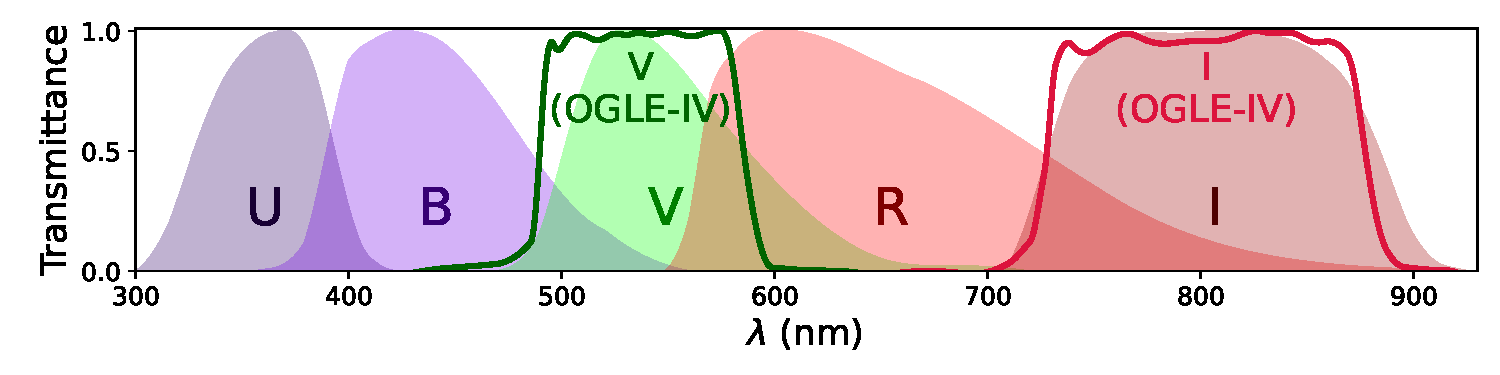
\includegraphics[width=\textwidth]{img/filters.pdf}
		\caption[Johnson-Cousins and OGLE-IV photometric systems]{
			Johnson-Cousins (filled) and OGLE-IV equivalent (solid) filters transmittance curves. 
			Colors are meant to be representative, not exact. UBVRI curves were adapted from \cite{Bessell2005}, and OGLE-IV curves from \cite{OGLE2015}. 
			It is to note that OGLE-IV curves are experimental measurements of custom made filters.
		}
		\label{fig:filters}
	\end{figure}
	
	\begin{table}
		\centering
		\begin{tabular}{c|c||c|c}
			Filter & description & $\lambda_{eff}$ (nm) & $\Delta_{\lambda}$ (nm) \\ \hline\hline
			U & Ultraviolet & 366.3 & 65 \\ 
			B & Blue & 436.1 & 89 \\ 
			V & Visual & 544.8 & 84 \\ 
			R & Red & 640.7 & 158 \\ 
			I & Infrared & 798 & 154
		\end{tabular}
		\caption[Johnson-Cousins effective wavelengths and bandwidths]{
			Effective wavelengths and bandwidths for the Johnson-Cousins photometric system. Data from \cite{Bessell2005}.
			}
		\label{tab:filters}
	\end{table}
	
	Absolute magnitudes for an object in these standard filters are presented as a sub-index: $M_B$ would be the blue absolute magnitude.
	Relative magnitudes are presented as the filter letters: $B$ would be the blue apparent magnitude.
	
	If the transmittance function of a filter \enquote{X} is denoted $T_X(\lambda)$, the apparent magnitude $X$ is physically obtained by the process
	
	\begin{equation}
		X = \int_0^\infty T_X(\lambda) R(\lambda) F(\lambda) \,d\lambda
	\end{equation}
	
	where $F(\lambda)$ would be the monochromatic flux (the light spectrum) of the star, 
	and $R(\lambda)$ would be the optical response of the instrumental system used to take the measure, without the filter
	\footnote{this would include things like the optical response of the telescope and mirrors, 
	and in the case of CCD detectors, the quantum efficiency, and a term $\frac{\lambda}{hc}$ for the photon counting process \citep{Bessell2005}.}.
	This process is rarely dealt with in a theoretical manner; 
	rather it serves here as a conceptual tool to understand what is going on where the measure is taken.
	
	\subsubsection{Color, extinction, and the Wesenheit index}
	
	The dimming of light intensity by effects of the distance has been discussed, and reached conclusion on \autoref{eq:distance-modulus}.
	But that equation is only valid if the light from the distant object is completely unperturbed.
	Even ignoring atmospheric or instrumental effects on that light, 
	the interstellar medium will have a considerable impact on the amount of light that reaches the detector,
	as the dust and gas absorbs and scatters the starlight. 
	
	This absorption would have a multiplicative effect of the flux, making it dimmer, 
	and therefore an \textit{additive} effect on the magnitude, because magnitudes are an inverse scale \citep{Karttunen2017}.
	Continuing with the filter X example, if we denote extinction-free quantities by the subscript 0, 
	and this additive extinction on the filter X by $A_X$, we have the full extent of \autoref{eq:distance-modulus}:
	\begin{equation}
		X = X_0 + A_X = M_X + 5 \log\left(\frac{r}{10 \text{ pc}}\right) + A_X \label{eq:extinction-distance-modulus}
	\end{equation}
	Astronomers define color indexes between pairs of filters as the difference on apparent magnitudes. Using \autoref{eq:extinction-distance-modulus}
	\begin{equation}
		X - Y = (M_X - M_Y) + (A_X - A_Y) = (X_0 - Y_0 )+ E(X-Y) \label{eq:color-index}
	\end{equation}
	where $X_0-Y_0$ is called the extinction-free color index, sometimes denoted $(X-Y)_0$,
	and $E(X-Y) = A_X - A_Y$ is called the color excess. 
	
	The ratio of total-to-selective extinction is defined for the filter $V$ as $R_V = A_V/E(B-V)$. 
	Experimentally it is known that its value can vary from 2.6 to 5.5 \citep{Clayton1988},
	but it is widely taken as its mean value of 3.1 in the interstellar medium, which is valid for the Magellanic Clouds \citep{Cardelli1989,Gorski2020}.
	
	If for a color index $X-Y$ and for a certain star, $R_{X-Y} = A_Y/E(X-Y)$ is known, 
	the so called extinction-free Wesenheit\footnote{
		German word for \enquote{essentiality, essential being}, 
		philosophical term for the fundamental identity of things \citep[page 341]{German1997}.
	}
	index \citep{Madore1982} is defined as
	\begin{equation}
		W_{X-Y} = Y - R_{X-Y} (X-Y) \label{eq:wesenheit}
	\end{equation}
	which upon expanding turns into
	\begin{align*}
		W_{X-Y} &= Y_0 + A_Y - \frac{A_Y}{A_X - A_Y}[ (M_X-M_Y) + (A_X - A_Y) ] \\ 
		&= Y_0 - \frac{A_Y}{A_X - A_Y} (M_X-M_Y)  \\ 
		&= Y_0 + R_{X-Y}(X-Y)_0 
	\end{align*}
	and thus is indeed free of extinction effects. Through this work, we will use the $V-I$ color index, and the Wesenheit index:
	\begin{equation}
	W_I = I - R_I (V-I) \label{eq:wesenheit-i}
	\end{equation}
	Where $R_I = \frac{A_I}{E(V-I)} = \frac{A_I}{A_V - A_I}$. 
	Similarly to the $R_V$ case, $R_I$ has a wide range of values on the literature, even with $R_V=3.1$ fixed \citep[for a discussion see][]{Nataf2015}. 
	It was measured in the Galactic bulge as $1.080\pm0.007$ by \cite{Pietrukowicz2012}. 
	Using the tables from \cite{Schlegel1998} and \cite{Schlafly2011} yields $1.411$ and $1.217$ respectively, for the Landolt filters.
	The first direct OGLE measurement of $A_I$ and $E(V-I)$ on the Magellanic system has a star-number weighted mean of $1.57\pm0.33$.
	Through the OGLE literature a value of 1.55 has been widely used \citep[see for instance][]{OGLE2015,Udalski1999,Ulaczyk2013},
	and thus we will use that value,
	but from the latest reddening maps, \cite{Reddening2021} derived $R_{I;SMC}=1.74$ and $R_{I;LMC}=1.67$.
	Actually, this $R_I$ should be calculated on a star-by-star basis, using those reddening maps,
	but that lies outside the scope of this work.
	
\subsection{Phase diagrams}

	\begin{figure}
		\centering
		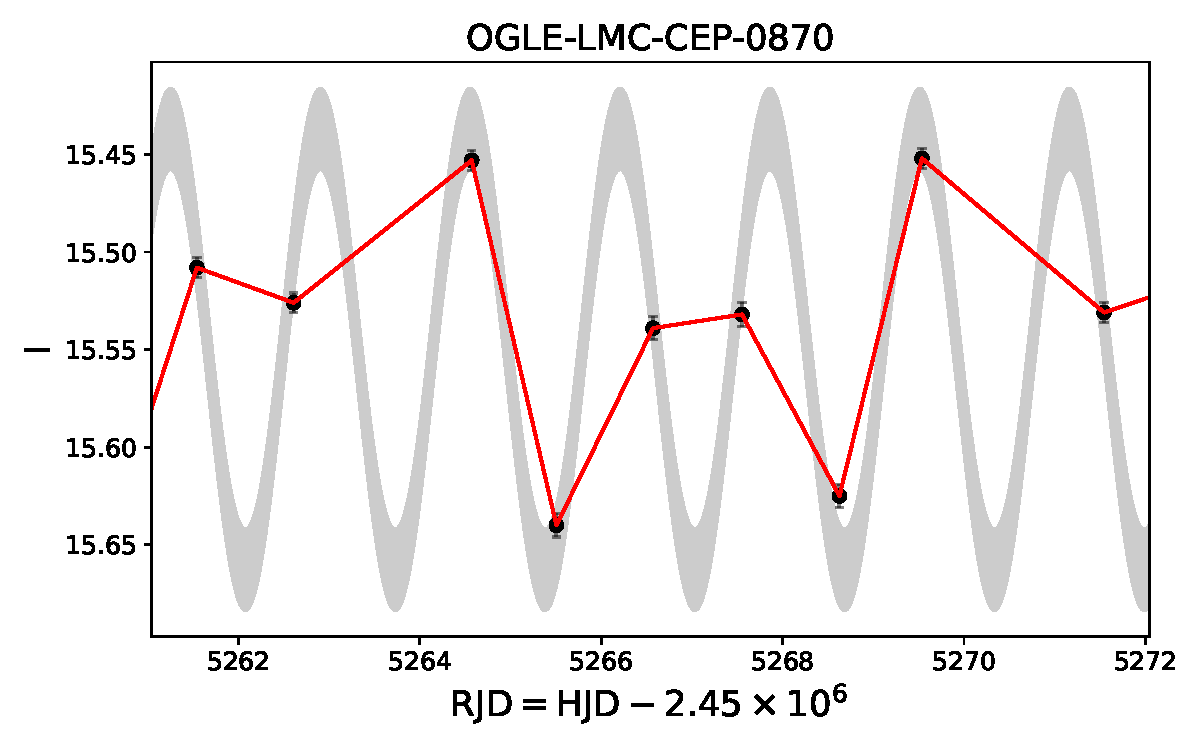
\includegraphics[width=0.7\textwidth]{img/interpolation_failure.pdf}
		\caption[Failure of interpolation of a light curve]{
			First points of the I band time series for a randomly selected star with low period from the OGLE database \citep{OGLE2016}.
			Data points are in black, and the actual light curve (Fourier series fit to all data) is shown as a gray band. 
			Simple interpolation is shown in red, showing that there is not enough data for a point-by-point interpolation to represent the underlying function.
		}
		\label{fig:interpolation-failure}
	\end{figure}

	With time and magnitude scales covered, the last definition needed is that of the phase. 
	Astronomical observations taken from the earth surface, ignoring those of the sun, can obviously only taken at night.
	Atmospheric related distortions are less prominent near zenith, 
	so measurements are ideally taken when the star is in its highest point in the sky,
	but telescope times are heavily scheduled, so the measure will be taken whenever possible.
	Additionally, because of the rotation of the earth around the sun, 
	there will be months of the year when the object will not be visible during night.
	
	These irregularities in the measuring times, apart from having consequences on the signal analysis process of the data,
	can obfuscate the phenomenology of the star's light curve, specially if its variability period is on the order of days.
	Continuous measurements $I_{t=0}$,$I_{t=1}$ (approximately one day apart) are not necessarily in the same period, 
	and thus there is no way to grant that the value at an intermediate time (say $I_{t=1/2}$) is even inside the $[I_0,I_1]$ range;
	any interpolation would eventually fail, as it is seen in \autoref{fig:interpolation-failure}.
	

	But as already stated, the shape of the light curve carries phenomenological details about the star variation.
	In order to recuperate that shape without having to fit the data, and if the period is known,
	one can define the \textit{phase} $\phi$ of a certain time $t$ as
	\begin{equation}
		\phi(t) = \frac{\text{mod}(t-t_0,P)}{P} = \text{mod}_1\left(\frac{t-t_0}{P}\right) \label{eq:phase}
	\end{equation}
	where $t_0$ is called the ephemeris time, and is commonly taken as the point with maximum brightness (minimum magnitude).
	The first definition is just the time that has passed since the last maximum divided by the period, 
	and the second is the fractional part of the time since \textit{any maximum}\footnote{
		By properties of the mod function, the phase remains the same if $t_0$ is shifted by any whole multiple of $P$.
	} in units of $P$.
	
	A phase diagram is then a plot of the phase against the magnitude. 
	Examples can be found on \autoref{fig:mag-phase-1} and \autoref{fig:mag-phase-2}.
	
	The condition that the period has to be known to properly make a phase diagram can seem ridiculous, 
	since the purpose of this work is to find periods.
	But this ends up playing in our favor: 
	it is precisely the fact that phase diagrams are only correct in the period that will allows us to find the period using phase diagrams.
	The discussion about how the phase diagram behaves on a wrong period and how that can be used to find the correct one is presented on \autoref{sec:phase-diagram-methods}.
	
	\begin{figure}
		\centering
		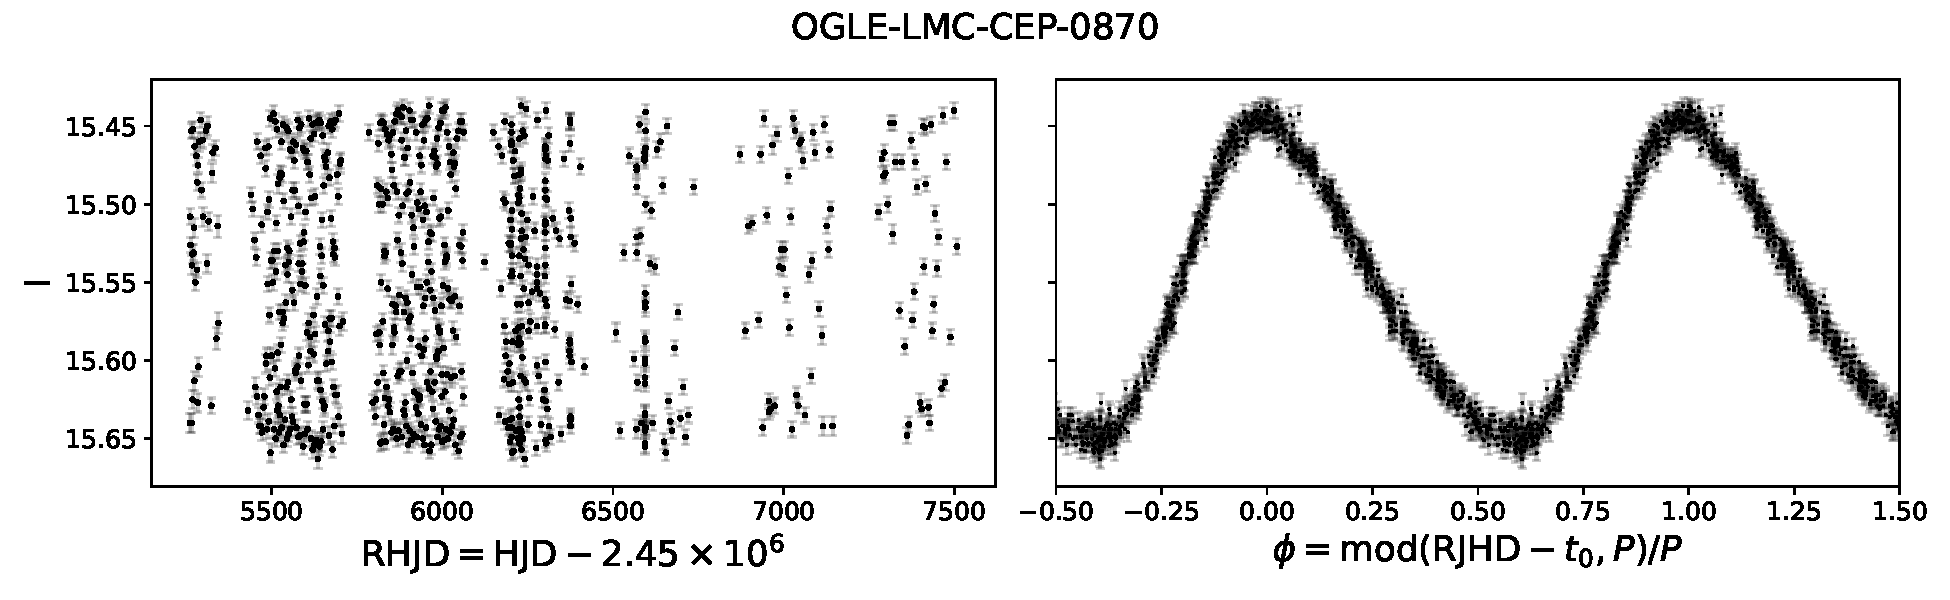
\includegraphics[width=\textwidth]{img/mag_phase_LMC_0870.pdf}
		\caption[Light curve of OGLE-LMC-CEP-0870]{
			I band time series and phase diagram for a randomly selected star with low period from the OGLE database \citep{OGLE2016}.
			Uncertainties for the magnitudes are shown as light gray error bars.
			Temporal units are ephemeris days, and ephemeris time $t_0$ is taken as the time with minimum magnitude.
			A period of $P=1.6518$ days was used for the phase.
			The yearly windows when the object cannot be observed from the ground observatory are clearly present in the time series.
		} 
		\label{fig:mag-phase-1}
	\end{figure}
	
	
	\begin{figure}
		\centering
		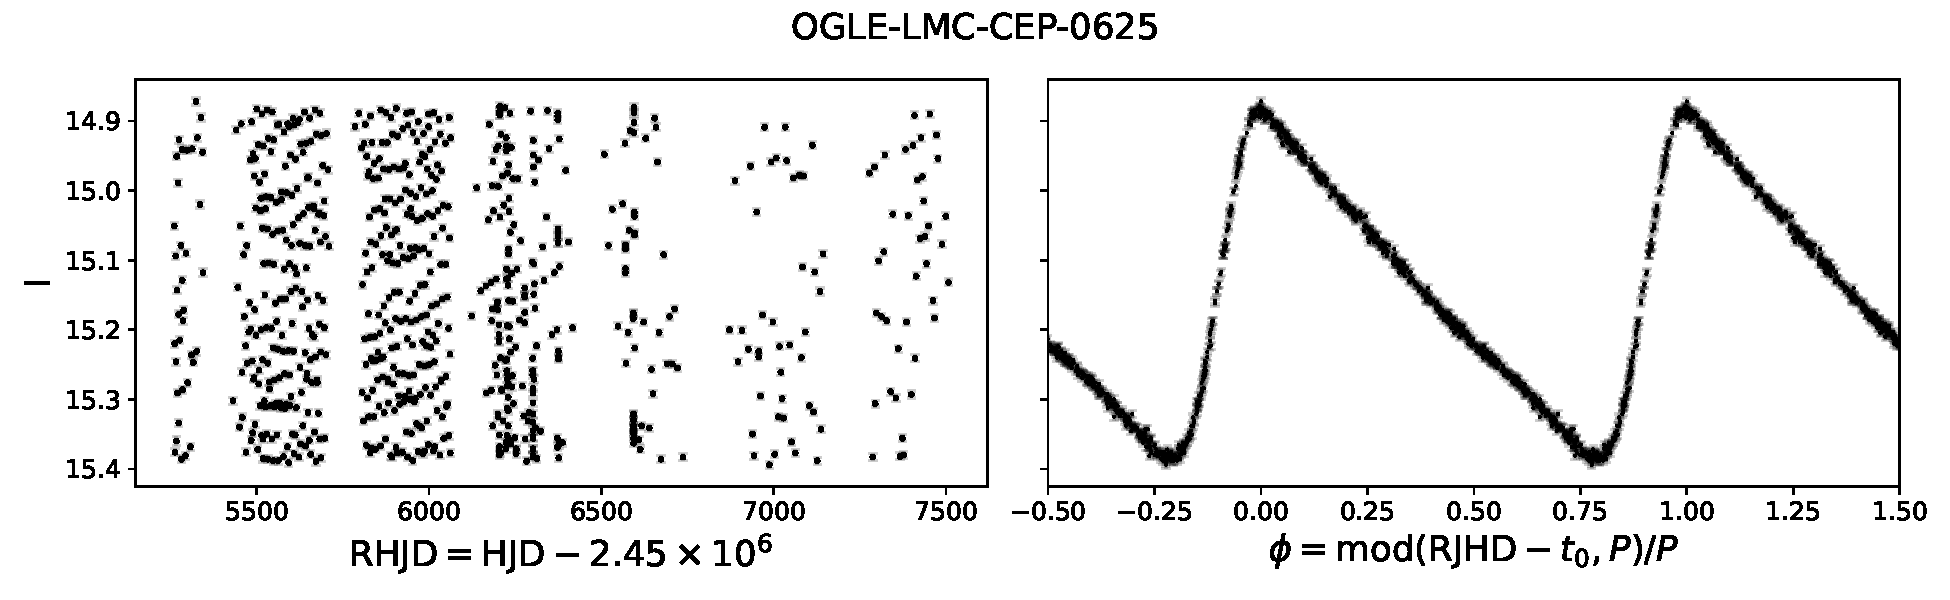
\includegraphics[width=\textwidth]{img/mag_phase_LMC_0625.pdf}
		\caption[Light curve of OGLE-LMC-CEP-0625]{
			Same as in \autoref{fig:mag-phase-1}, but for a typical Cepheid in the LMC. 
			A period of $P=3.7503$ days was used for the phase.
			Phases are padded cyclically for values outside the $[0,1]$ range for clarity, to better observe the behavior of all parts of the light curve.
			Data from \cite{OGLE2016}. 
			A notable difference of this figure and \autoref{fig:mag-phase-1} is the amount of \enquote{dispersion} or width of the light curve.
			This dispersion is much larger than the experimental uncertainty, and should be intrinsic to the star, 
			a phenomenon which deserves further study.
		}
		\label{fig:mag-phase-2}
	\end{figure}
	
	
\section{Cepheid Variable stars}
	
	Classical Cepheid are radial pulsating variable stars, 
	named after the prototypical $\delta$ Cephei as discussed in \autoref{sec:intro-stellar-variability}.
	But that can be a bit misleading, 
	as the term actually refers to an evolutionary stage that some stars present even multiple times in their lifespan.
	Some stars (depending on their mass) leave the main sequence as their Hydrogen fuel gets consumed,
	and evolve into what is known as the instability strip (see \autoref{fig:HR-diagram-karttunen}).
	Cepheids are yellow giants or supergiants at this point \citep{Catelan2015}, and began to experience radial pulsation,
	typically with a period of 1 to 50 days, changing their brightness with amplitudes ranging from 0.1 to 2.5 magnitudes,
	and going from spectral type F to G or even K \citep{Karttunen2017}.
	Their masses can vary from $\sim1 M_\odot$ to $20 M_\odot$, and their radius from $\sim10R_\odot$ to $200R_\odot$
	
	The former are the characteristics of galactic Cepheids, 
	but it is known that there are extra-galactic Cepheids with shorter and larger periods, 
	specially in the Magellanic system \citep{Payne1967,Cox1980}. 
	The data taken by the OGLE project is in agreement with that ranges; see \autoref{sec:data} for more details.
	
	
	\begin{figure}
		\centering
		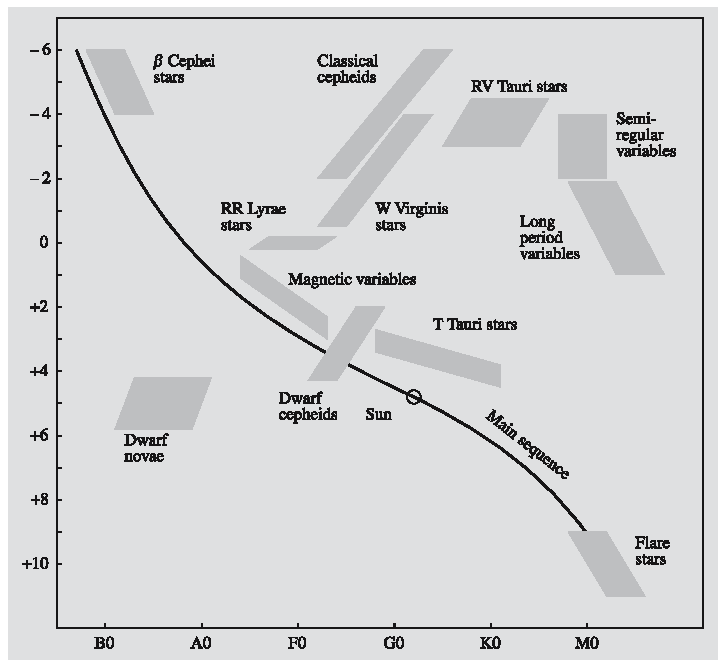
\includegraphics[width=0.7\textwidth]{img/Karttunen_13.2.pdf}
		\caption[Variable stars in the HR diagram]{
			Position of several types of variable stars in a Hertzsprung-Russell diagram.
			The abscissa is given as spectral class, proportional to temperature and color: 
			red (cooler, 3750 K at M0) on the right and blue-white (hotter, 27000 K at B0) to the left. 
			The ordinate is given in absolute visual magnitude $M_V$.
			The main sequence is represented as a solid line, and the Sun as a circle.
			Classical Cepheids can be seen on the red giant branch. 
			Taken from \cite{Karttunen2017}, Figure 14.2.
		}
		\label{fig:HR-diagram-karttunen}
	\end{figure}
	
	\subsection{Stellar populations}
	
	Stars contents are generally classified percentually as Hydrogen ($X$), Helium ($Y$) and \enquote{metals} ($Z$), 
	that constitute really any other element present in the star\footnote{
		For reference, the current surface values for the sun are $X=73.81\%,\,Y=24.85\%,Z=1.34\%$ \citep{Asplund2009}.
	}.
	As the nuclear fusion in the star core turns Hydrogen into Helium, and Helium into heavier elements up to Iron, 
	the balance of the mass fractions over the stars moves from $X$ to $Y$ and eventually to $Z$ as the time passes.
	Moreover, massive stars die in cataclysmic events known as novæ, which have the energy to produce metals heavier than Iron.
	As new stars form from the remnants of the old ones, they have a greater amount of metals from the beginning, 
	but early stars on the Universe would have been mostly Hydrogen, the simplest element.
	
	The idea of the stars coming in generations is attributed to Oort, according to \cite{Baade1944}.
	Baade classified as population I the high metallicity ones (modern value $Z\approx 2\%$), the youngest, 
	and population II the oldest (modern value $Z\approx 0.1\%$) \citep{Carroll2017}. 
	A population III have been theorized since then, those of the first generation of stars, but none have been observed \citep{Heger2002}.
	There is a discussion around the timescales needed for the violent death of the stars to occur (specifically type Ia supernovæ), 
	and if it is sufficient to produce the metallicity difference among populations \citep{Carroll2017}.
	Regardless, the PL relations are dependent on population, and in this work only Cepheids of population I will be considered.
	
	
\subsection{Radial stellar pulsation}
	
	\subsubsection{The period-density relation}

	The most intuitive way of interpreting the radial pulsations of a star 
	is by considering sound-like waves traveling from its center to its surface.
	As a crude approximation, we could consider the equilibrium at the last layer of a star of total mass $M$ and  radius $R$,
	say, a spherical shell of width $dr$ and mass $m\ll M$ at the limit $r\to R$ . 
	Assuming that the pressure outside of the star is zero, and the pressure just below our outer shell is $P$,
	there would be an outward force $P\,A=P\;2\pi r^2$ opposed by the gravitational pull $GMm/r^2$.
	This naive equation of motion would then be
	\begin{equation}
		m \ddot{r} = P 4\pi r^2 - \frac{GMm}{r^2} \label{eq:period-density-motion}
	\end{equation}
	After a painful process of linealization, we will get an equivalent to the Linear Adiabatic Wave Equation (LAWE):
	\begin{equation}
		-\frac{1}{r^4 \rho} \frac{d}{dr}\left(\Gamma_1P r^4 \frac{d\eta}{dr}\right) - \frac{1}{\rho r}\left(\frac{d}{dr}\left[\left(3\Gamma_1-4\right)P\right]\right)\eta = \omega^2 \eta \label{eq:lawe}
	\end{equation}
	where perturbations on $r$ of the form $\xi = \eta e^{i\omega t}$ have been considered, $\rho$ is the mean density and $\Gamma_1$ is the first adiabatic exponent\footnote{
		$\Gamma_1=5/3$ for an ideal gas, and it is the value recommended by \cite{Cox1980}. 
		Interestingly enough, $\Gamma_1=4/3$ for radiation, and the period actually diverges if one blindly uses \autoref{eq:period-density-relation}.
	}. This is equation~5.90 of \cite{Catelan2015}, where the whole linealization process can be consulted.
	\autoref{eq:lawe} is a more general form of that first derived by \cite{Eddington1918}.
	As already stated, the perturbations on the radius are assumed as outward waves with amplitude $\eta$ and angular frequency $\omega$.
	In our simplistic model, the amplitude does not depend on the position of the spherical shell, so $\frac{d\eta}{dr}=0$, and the first term vanishes.
	We shall take away all the radial dependencies, except of course for that of the pressure, as we are considering sound waves:
	\begin{equation}
		\left(\frac{3 \Gamma_1-4}{R\rho}\right)\left(-\frac{dP}{dr}\right) = \omega^2 \label{eq:lawe-result}
	\end{equation}
	That pressure dependence comes from the pressure gradient equation of stellar evolution (in its hydrodinamical from) \cite[equation 4.18]{Catelan2015}:
	\begin{equation}
		\ddot{r} = -\frac{1}{\rho} \frac{d P}{d r}-\frac{GM}{r^3}
	\end{equation}
	which we can use in equilibrium ($\ddot{r}=0$) on \autoref{eq:lawe-result} to get
	$$
	\omega^2 = (3\Gamma_1-4)\frac{GM}{R^3}
	$$
	And in terms of the period $\Pi$ and the mean density $\rho=M/(\frac{4}{3}\pi R^3)$
	\begin{equation}
		\Pi = \frac{2\pi}{\sqrt{(3\Gamma_1-4)\frac{4}{3}\pi G \rho}} \label{eq:period-density-relation}
	\end{equation}
	
	This is usually just a rough estimation of the order of magnitude of the period. 
	For instance, the parameters for $\delta$ Cephei would be $M=4.5\pm0.3 M_\odot$, $R=44.5R_\odot$ \citep{Matthews2012},
	which assuming ideal gas for $\Gamma_1$ gives $\Pi=16.2\pm0.5$ days. 
	The real period is $5.366249$ days \citep{Samus2017}.
	As seen below these oscillations are not necessarily adiabatic, and the amplitude should actually decay.
	

	\subsubsection{The Eddington valve and the $\epsilon$, $\kappa$ and $\gamma$  mechanisms \label{sec:eddington}}
	
	Through the 20th century \cite{Eddington1918,Eddington1926,Eddington1941} 
	proposed a thermodynamic cycle to be responsible for the radial pulsation of stars. 
	He devised two possible physical causes to drive this \enquote{valve}, known today as the $\epsilon$ and $\kappa$ mechanisms.
	
	The $\epsilon$ mechanism is based on the idea that the nuclear processes at the core of the star 
	are more intense in the contraction than in the expansion phase of the valve.
	This would increase the pressure of the stellar material in the contraction phase, 
	and decrease it in the expansion, working in a similar fashion as a Diesel engine \citep{Zhevakin1963}.
	Although it is true that nuclear reaction rates increase with temperature and pressure, 
	this effect only becomes dominant at higher masses ($\sim 100 M_\odot$) and is in fact destabilizing \citep{Carroll2017,Zhevakin1963,Catelan2015}.
	Thus, at least for Cepheids and related variable stars types, the $\epsilon$ mechanisms is not the primary source of radial pulsation.
	
	The second mechanism proposed by Eddington depends on the star stopping 
	the energy leakage from the nucleus when the star is compressed, and allowing that energy to leak when the star expands.
	If the energy is \textit{somehow} retained in the core when the star is contracted,
	the temperature and the pressure will raise, and the star will be forced to expand.
	If then, at the peak of the expansion, the star \textit{somehow} allows that nuclear energy to escape at a higher rate than normal,
	the temperature and pressure in the inside will drop, 
	and the gravitational pull would then win over the pressure gradient, 
	and force the system to began compression again, closing the valve's cycle.
	This would allow the star to pulse without depending on violent variations on the nuclear reaction rates.
	
	But those \enquote{somehow} are quite problematic. Kramers opacity law states that 
	the optical opacity of the stellar material behaves as $\kappa \propto \rho T^{-3.5}$ \citep{Carroll2017}.
	As the dependence is stronger with the temperature, the opacity in the compression phase would be lower, not higher.
	The opacity is directly proportional to the energy (radiation) absorption, and thus the system would not work as Sir Eddington expected.
	
	But there is a way for the temperature changes to be damped at compression and expansion on certain layers of the star. 
	These are called partial ionization zones, and are cause by the increase of degrees of freedom on Hydrogen and Helium gases undergoing ionization \citep{Cox1963},
	which effectively rises the heat capacities $C_V$ and $C_P$ of the layers \citep{Carroll2017}.
	There are two such layers, one where Hydrogen and Helium experience their first ionization:
	$$
		\left.\begin{matrix}
			\text{H I} &\to &\text{H II} & \text{at} & 13.5984345997(02\pm12) \text{ eV} \\
			\text{He I} &\to &\text{He II} & \text{at} &  24.5873890(90\pm25) \text{ eV}
		\end{matrix}\right\} \text{(first ionization)}
	$$
	and one deeper layer where the Helium experiences its second ionization:
	$$
		\text{He II} \to \text{He III}\quad \text{at}\quad 54.4177654(86\pm25) \text{ eV} \qquad \text{(second ionization)}
	$$
	Those energies \citep{NIST_ASD} put all those transitions in the ultraviolet region of the electromagnetic spectrum.
	The ionizations \enquote{leak} a fraction of the energy that otherwise would have been spent on increasing the temperature.
	As the temperature increase is less prominent, the density term in Kramers law dominates, and therefore the opacity increases.
	
	Conversely, in the expansion phase, the ions interact with free electrons, releasing energy that is absorbed by the gas, increasing the temperature.
	As the temperature drop for the expansion is less than expected, the density term dominates again, and the opacity decreases. 
	This two processes are known as the $\kappa$ mechanism, proposed by \cite{Zhevakin1963} and verified by \cite{Cox1963}.
	Moreover, the changes in the heat capacities and the damped temperature gradients causes more heat to flow into those layers,
	positively reinforcing the cycle in which is known as the $\gamma$ mechanism.
	
	The position and behavior of this layers is critically dependent of the temperature, and hence the instability strip discussed before must be almost vertical,
	as \cite{Cox1963} derived theoretically. This can be seen in the position of the Cepheid branch on \autoref{fig:HR-diagram-karttunen}.

	This effect also ---and finally--- explains the asymmetrical variability of the brightness on pulsating stars.
	The amount of luminosity retained by the partial ionization layers depends on their position,
	and it releases when the layers are propelled outwards and its opacity diminishes \citep{Carroll2017}.
	The more energy trapped on the compression phase, the greater the force that would make the star expand,
	and as the opacity has just decreased, the increase of brightness happens faster.
	On the other side, the gravitational pull and the pressure gradient that closes the cycle and causes compression again
	are slower, since all of that energy has escaped in the form of light. 
	
	% ascending and descending branches TODO
	
	% put astrophysical consideration of ascending branch in a caption, new figure TODO
	
	The consensus is that all of those mechanisms do require exceptional conditions to actually work, 
	and that could explain why stellar pulsators are indeed rare in the bulk population of stars in the Universe,
	being approximately one for each $10^5$ stars \citep{Carroll2017}.
	
	\subsubsection{Pulsation modes}
	
	% does a star change its pulsation overtones? TODO
	% polaris
	
	Returning to the intuition of the sound waves of the beginning of the section,
	one could be surprised to know that \autoref{eq:lawe} can actually be solve exactly.
	In fact, it constitutes an special case of what is called a Sturm–Liouville problem.
	As any other physics equation with similar generality, there is an infinite family of solutions,
	and we will not go into the details here; it can be consulted on \S 5.6 of \cite{Catelan2015},
	and more generally on \S  9.3 of \cite{Butkov1968}.
	
	But there are important conclusions derived from the solution of \autoref{eq:lawe}.
	In the first place, it is always the case that $\omega^2$ is a real number, but it can be negative, so $\omega$ is not always real.
	As the waves are defined with $e^{i \omega t}$, imaginary frequencies correspond usually to a cataclysmic behavior of the star.
	We will be concerned with the real frequency case, where the wave act as in oscillatory motion.
	This frequency is called the eigenvalue of the system, say $\omega_n$, and it is associated with an eigenfunction $\eta_n$.
	
	Those eigenfunctions act as basis functions for all the waveforms than could be present in the pulsation of the star,
	in a similar way as the sinusoidal functions act as a basis (the Fourier basis) for the sounds produced in a pipe or a flute.
	Moreover, in the same way a pipe can present harmonics with higher frequencies than its lowest standing wave, 
	each of the $\omega_n$, $n>0$, is a harmonic standing wave pulsating radially onto the star.
	
	Therefore it can (and will) be the case that a star is pulsating primarily in, say, the first harmonic ($\omega_1$), 
	or a combination of the fundamental ($\omega_0$) and other harmonics.
	This is denoted as \texttt{nO}, where \texttt{n} is the harmonic (or Overtone, \texttt{O}) number. The \enquote{zeroth} overtone is denoted \texttt{F}, for Fundamental.
	For instance, a star pulsating in its fundamental and second overtone would be denoted \texttt{F2O}. A first and second and third overtone pulsator would be \texttt{1O2O3O}.
	
	The direct solutions of \autoref{eq:lawe} would be of little to no use for this work, 
	as the observational data only includes the magnitude variation, 
	and it is difficult to translate that into radial motion.
	Nevertheless, in the following section will be described how to analyze the magnitude variability using the Fourier theory, and some additional methods.
	
	
\section{The other spectrum, the pulsation spectrum}

If we wanted to extract information from a periodic signal, 
the most natural thing to do is to check how the signal \enquote{correlates} with certain frequencies.
The pure, ideal, harmonic oscillator would correlate only with a single frequency,
but more complex phenomena could correlate with several frequencies with different intensities,
as if one were to describe several coupled oscillators in terms of their normal modes.

This \enquote{correlation} is not precisely defined at this point, but left as an intuitive concept.
This is done purposefully, as we will present several ways to measure it.
Any function that express the intensity of the correlation of a given signal with a frequency as independent variable
would be called a power spectrum. The terms \textit{spectrogram}, \textit{Fourierogram} and \textit{periodogram} are also used through the literature.

\subsection{Fourier Analysis}

When we say frequency, we mean frequency $\nu$ of uniform rotation in some space, as described by a simple waveform $e^{2i\pi \nu t}$.
The decomposition of a function into a linear combination of regular rotations must be based in the theory of Fourier analysis,
if interrogated well enough. 

Then, we will define the basics of the theory. If we have a theoretical signal $f(t)$, that is mathematically well-behaved,
its representation in frequency space would be given by the function
\begin{equation}
	F(\nu) = \int_{-\infty}^\infty f(t) e^{2\pi i \nu t} dt \label{eq:fourier-transform}
\end{equation}
and its called the Fourier transform. The inverse transformation is given by 
\begin{equation}
	f(t) = \int_{-\infty}^{\infty} F(\nu) e^{-2\pi i \nu t} d\nu
\end{equation}
where we follow the conventions from \cite{Deeming1975}. In general, $F(\nu)$ would be a complex number.
The canonical power spectrum is defined as its magnitude:
\begin{equation}
	P(\nu) = F^\ast(\nu) F(\nu) \label{eq:conjugate}
\end{equation}


	\subsubsection{Discrete non-uniform Fourier transform}
	
	One could be purely practical and force the discretization of \autoref{eq:fourier-transform} to a signal with data $\{t_k,f_k\}$,
	defining $f(t) = \sum_k f_k \delta(t-t_k)$, but I propose to deduce it by a visual construction, building it up from the phase diagram.
	
	In \autoref{eq:phase}, the phase was defined as a dimensionless number; the fraction of the period elapsed since the last maximum.
	As an amount of time relative to the period, it goes from 0 to 1.
	We can translate that to a rotational motion interpretation, by making that temporal phase $\phi$ into an angular one $\psi=2\pi \phi$,
	as if that phase were not seen as the fraction of a period, but as the fraction of a rotation.
	This is made to eliminate the need for a modulus operation. For each data point, our definitions would be
	$$
	\phi_k = \frac{t_k-t_0}{P} = \frac{\omega}{2\pi}(t_k-t_0) \qquad \psi_k = \omega(t_k-t_0)
	$$
	That way, the angular phase $\psi_k$ corresponds to the argument of a typical sinusoidal function $\sin(\omega(t_k-t_0))$.
	The phase diagram was a (temporal) phase against magnitude plot, but we can construct a polar plot with these $\phi_k$ as angles and the magnitudes ($f_k$) as radii.
	Such comparison of linear-to-angular representations can be seen in \autoref{fig:complex-phase}.
	One could call this polar plot a \enquote{Fourier curl}, or also a \enquote{complex phase diagram};
	as it is composed of the points $\{f_k \cos(\omega(t_k-t_0)),f_k \sin(\omega(t_k-t_0))\}$, 
	anyone would be tempted to just define it using Euler's formula in the complex plane as $f_k e^{i \omega (t_k-t_0)}$.
	
	\begin{figure}
		\centering
		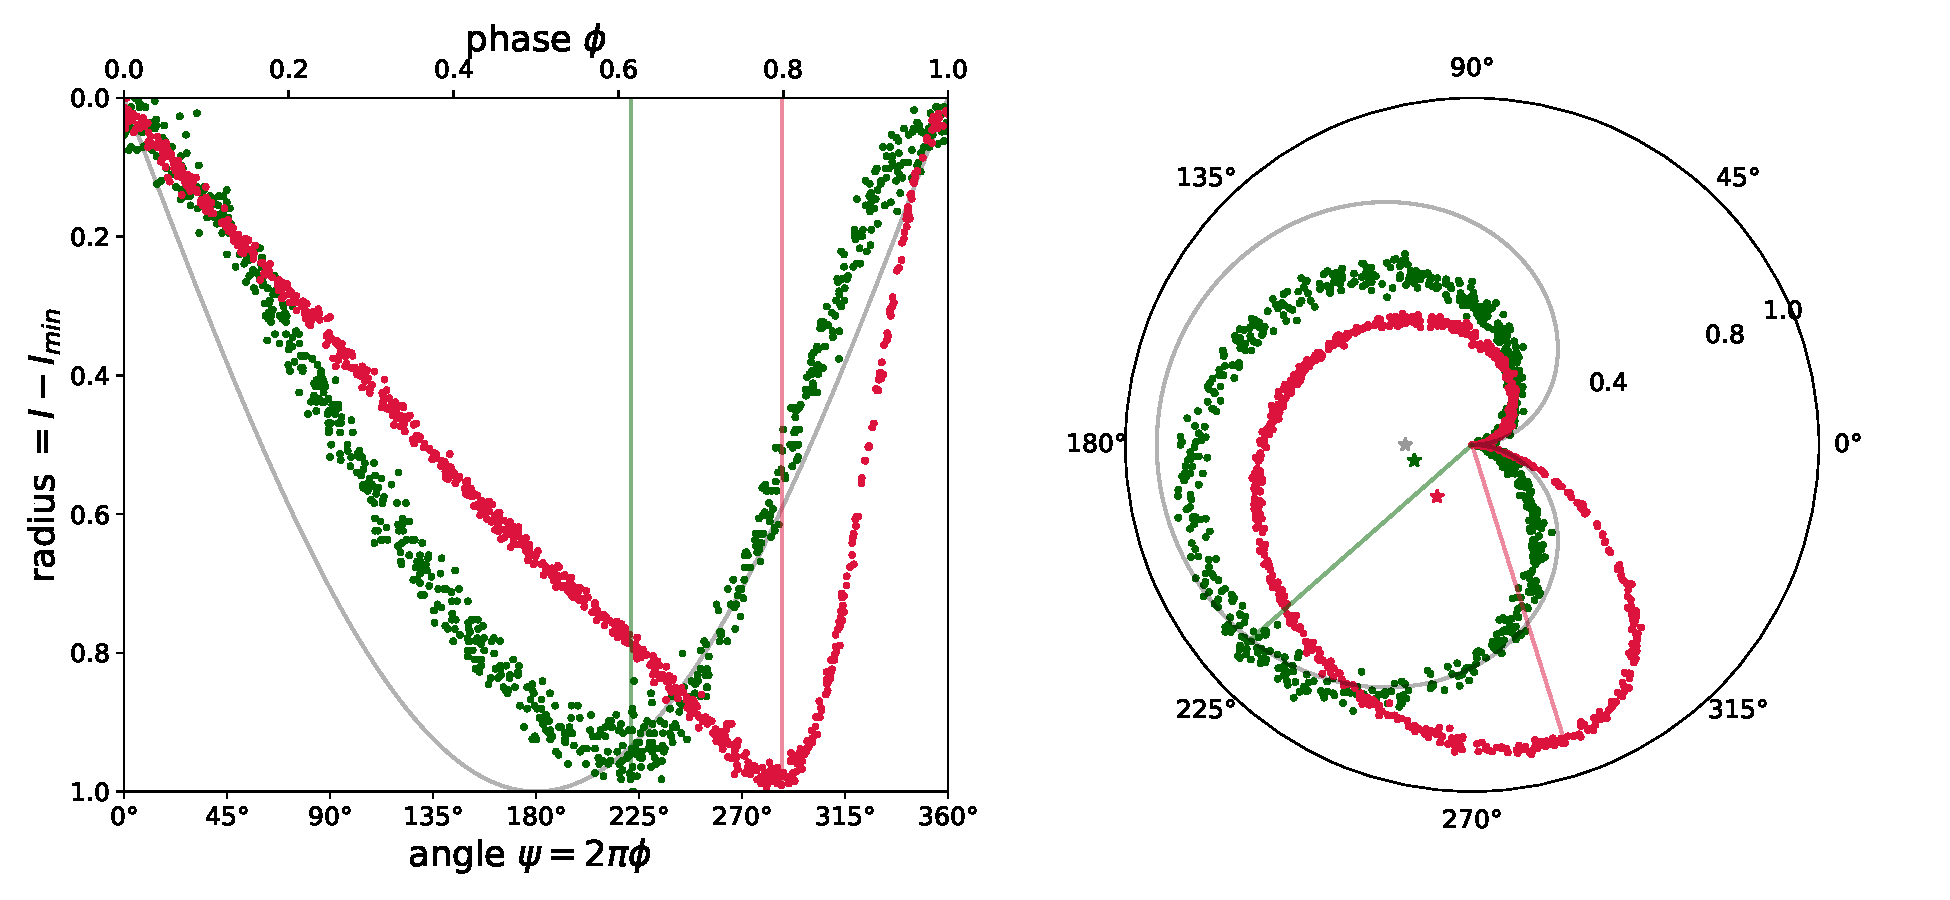
\includegraphics[width=\textwidth]{img/complex_phase.pdf}
		\caption[Complex phase diagram: Fourier curl]{
			Normal and polar phase diagrams for the sample stars in \autoref{fig:mag-phase-1} and \ref{fig:mag-phase-2}, 
			in green and magenta respectively. A simple sine curve is shown in light grey as reference.
			The magnitude was normalized to the $[0,1]$ range for visibility. 
			In the phase diagram, brighter is up. In the polar diagram, brighter is towards the center, and dimmer the larger the radius.
			A transparent line was drawn from the zero of each axis to the point of minimum brightness, for reference.
			In the polar plot, a $\star$ sign represents the centroid of each of the curled data.
			It is of note how the symmetric sinusoid curls up to a cardiod.
		}
		\label{fig:complex-phase}
	\end{figure}
	% augment with off phasing like \ref{fig:offphase} TODO 
	% row of phase
	% row of polar
	
	If the data were to be flat, or just random, one would expect the points in the polar plot to be distributed on an uniform fashion.
	On the opposite case, when the signal is just a sine wave, the polar figure would be a cardioid. 
	The middle case of just a periodic function with relatively low noise is pictured in \autoref{fig:complex-phase}.
	There is a definite clump of points in one direction.
	The most natural way to discern between noise and patterns in this case would be to look at the centroid of the curled figure. 
	In the complex plane this is just the mean of the points:
	\begin{equation}
		C = \frac{1}{N}\sum_{k=1}^N f_k e^{i \omega (t_k-t_0)} \label{eq:centroid}
	\end{equation}
	If we drop the $1/N$ factor and the ephemeris $t_0$, and express it in normal frequency terms $\nu=\omega/(2\pi)$, we get the general discrete Fourier transform:
	\begin{equation}
		F(\nu) = \sum_{k=1}^N f_k e^{2\pi i \nu t_k} \label{eq:fourier}
	\end{equation} 
	as defined by \cite{Deeming1975,Thomson1971,Schuster1898}. 
	The power spectrum in this case would be proportional to the magnitude of the centroid of the Fourier curl, 
	and therefore the independence from $t_0$ is justified.
	
	Provided that there are enough points, and perhaps more importantly, sufficiently wide in time, 
	if $\nu$ were not to be the correct frequency for the signal, the polar plot would be misaligned.
	That is, it would have several \enquote{petals} along all angles, like a rose curve,
	which means that the centroid would be displaced towards the center, its magnitude becoming smaller.
	The more \enquote{correlation} a signal has with a given frequency, the better the alignment of the figure in the polar plot;
	the points with larger radii will clump to one side, and the magnitude of the centroid will be maximum, as can be observed in \autoref{fig:complex-phase-off}.
	
	\begin{figure}
		\centering
		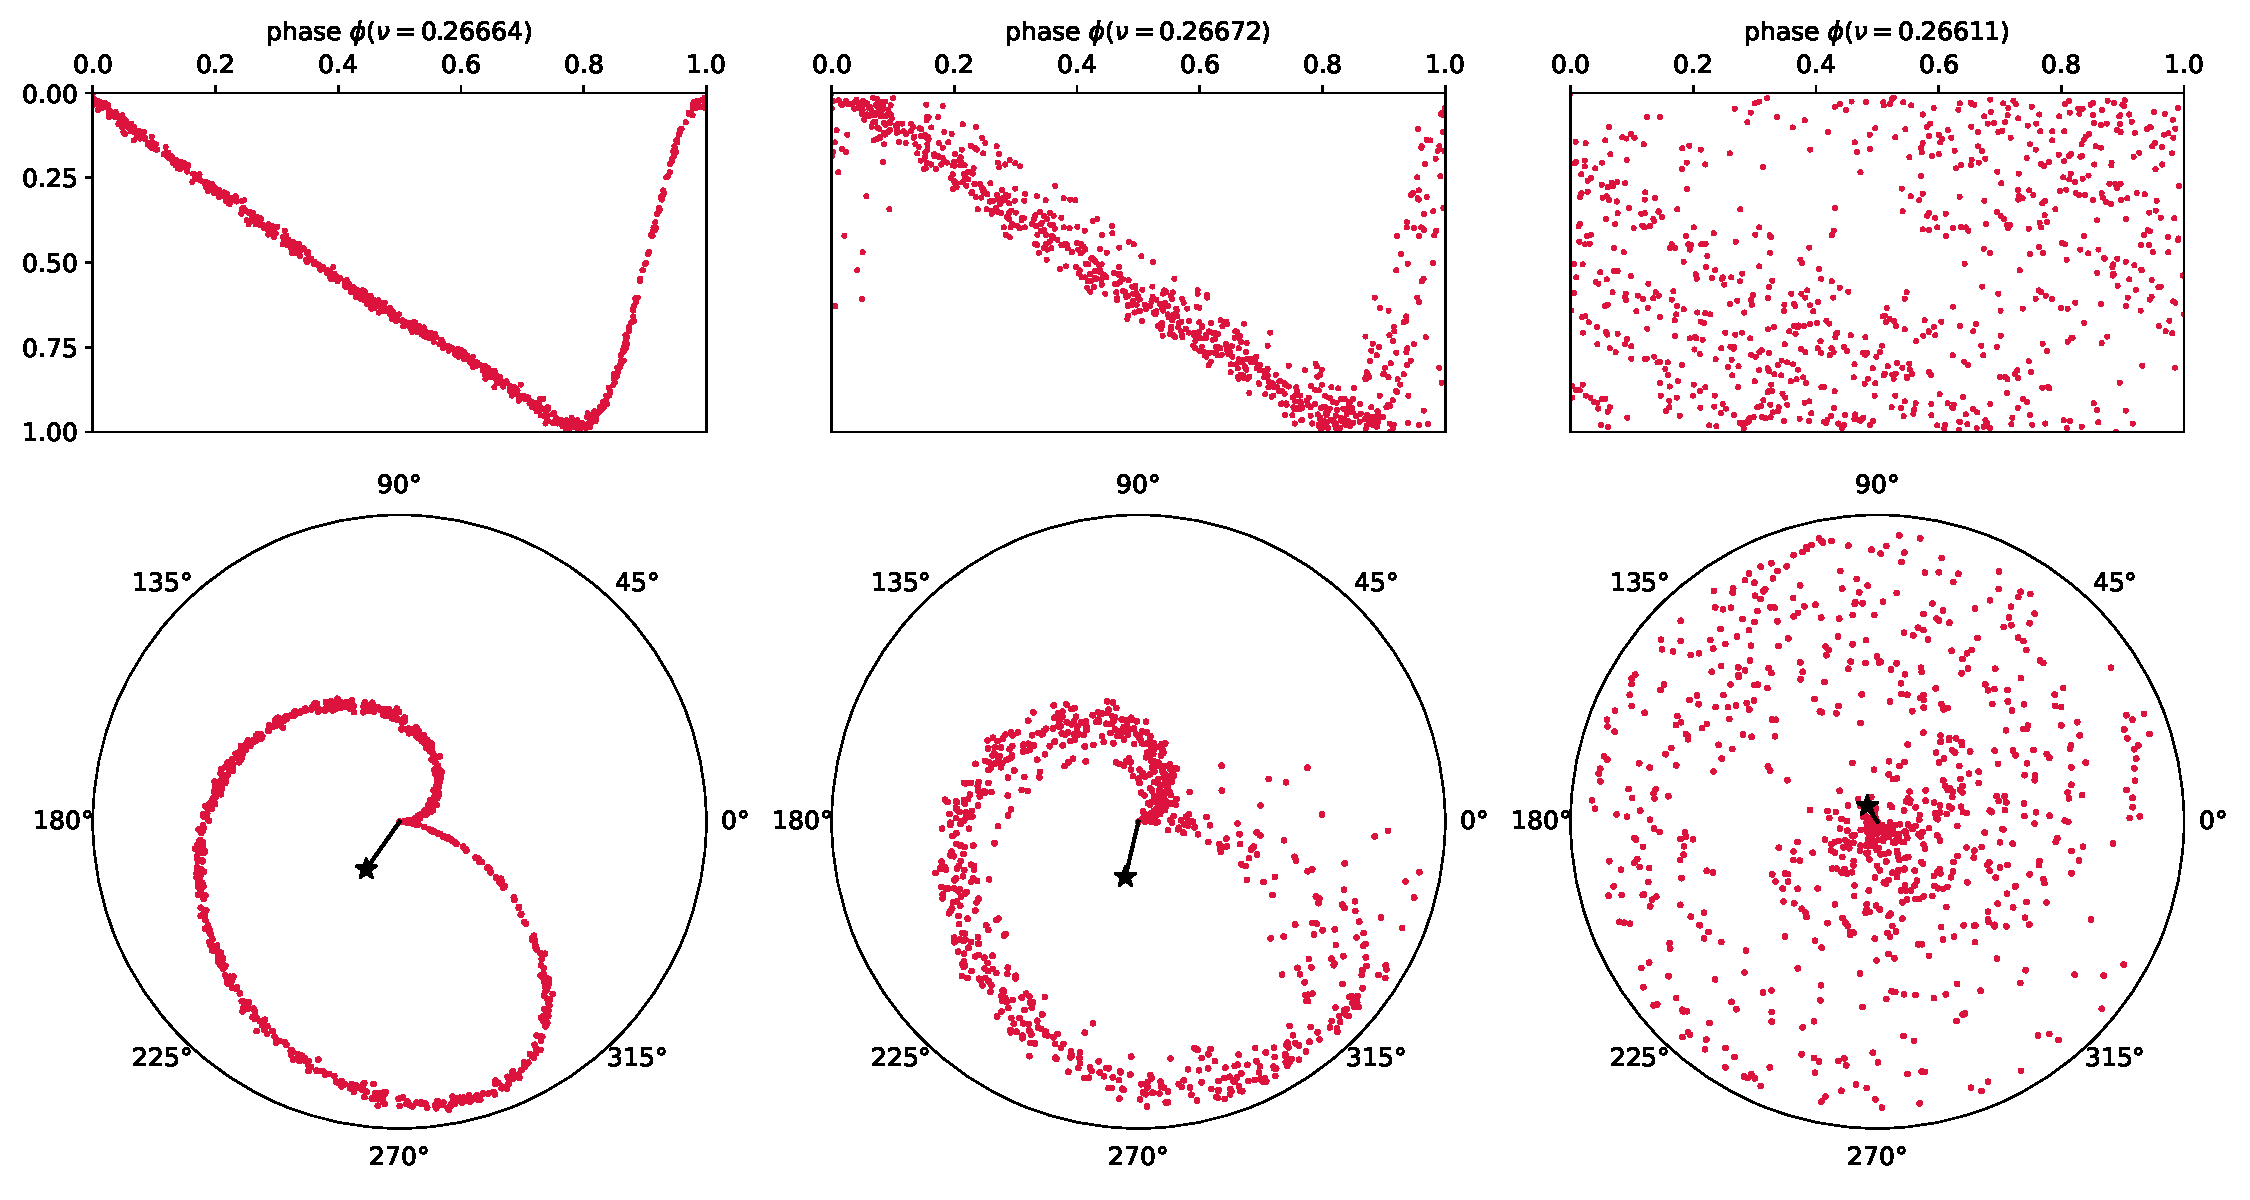
\includegraphics[width=\textwidth]{img/complex_phase_off.pdf}
		\caption[Off-frequency phase diagrams: real and complex]{
			Several phase diagrams (Fourier curls) calculated with different sample frequencies for the star in \autoref{fig:mag-phase-2}.
			Each colum has the normal phase diagram and the polar one. A black line and a star ($\star$) symbol represents the centroid of the curled figure.
			The first column has the correct frequency, and thus the points are clumped together.
			The second column has a frequency only slightly higher; the figure begins to misalign, 
			but the magnitude of the centroid is mostly stable: this periodogram is not as sensitive as the others.
			The las column has a \enquote{completely wrong} phase, despite having two correct decimals.
			The data is distributed more or less uniformly along the angles, and therefore the centroid is almost at zero.
		}
		\label{fig:complex-phase-off}
	\end{figure}
	
	A power spectrum calculated this way would have a peak at the principal frequency, and smaller peaks in the harmonics of the signal.
	In theory, these peaks of the power spectrum are invariant over scale changes, 
	but in practice their widths and heights would depend on the particularities of the data.
	
	As this method involve just a sum over the data, it is expected to be $O(n)$,\footnote{
		All time complexities are given per single frequency iteration. 
		Calculating an spectum with $f$ frequencies, the complecity of a single iteration have to be multiplied by $f$.
	} 
	with an overhead due to the complex exponential (or trigonometric) calculations.
	
	But the most important properties of this way of defining the Fourier power spectrum, in contrast with the fast Fourier transform (FFT),
	is the ability to be evaluated in any frequency $\nu$ with some freedom on the sample times $t_k$\footnote{
		There are some limitations in the reliability of the spectrum depending on the sampling frequencies \citep{Marvasti2001},
		but nonuniform sampling seems to mitigate the problem, as will be discussed in \autoref{sec:sampling}.
	}. 
	The FFT requires the data to be evenly spaced on time, and it calculates the power spectrum on an evenly spaced frequency grid \citep{Brigham1974}.
	As we will see in \autoref{sec:data}, astronomical terrestrial data is far from being evenly sampled, 
	and \autoref{fig:interpolation-failure} already stated that interpolation is not an option either.
	
	
	\subsubsection{The Lomb-Scargle periodogram}
	
	Apart from the very theoretical definition of the correlation between a signal and a frequency that we just presented,
	there is an even simpler one. We could define the correlation of the signal $\{t_k,f_k\}$ with a frequency $\nu$ as 
	how well does the signal is fitted by the model
	$$
	f_k + \epsilon_k = A \cos(2\pi \nu t_k +\phi)
	$$
	where $\epsilon_k$ are independent, normally distributed error terms, and $A$ and $\phi$ are the model parameters.
	In the literature the model is often presented as $A\sin(\omega t_k)+B\cos(\omega t_k)$, 
	which is completely equivalent, as both are forms of a first order Fourier series.
	After the least squares minimization, the coefficient of determination of the fit is given by \citep{Lomb1976,Scargle1982}
	\begin{equation}
		R^2(\omega) \propto \frac{\left(\sum_j f_j \cos\omega (t_j-\tau_\omega)\right)^2}{\sum_j \cos^2\omega(t_j-\tau_\omega)}+
		\frac{\left(\sum_j f_j \sin\omega (t_j-\tau_\omega)\right)^2}{\sum_j \sin^2\omega(t_j-\tau_\omega)} \label{eq:lomb-scargle}
	\end{equation}
	with
	\begin{equation}
		\tau_\omega = \frac{1}{2\omega}\arctan\left(\frac{\sum_j \sin 2 \omega t_j}{\sum_j \cos 2 \omega t_j}\right)  \label{eq:tau}
	\end{equation}
	This $R^2$ can be thought as a first order approximation of the Fourier spectrum, as is lacking the high order terms,
	but it is good enough to discern the peaks of the spectrum.
	%Because of that, this spectrogram is less noisy, something that could be preferred in some cases.
	
	Cepheid light curves, though, are typically not that sinusoidal, as we have established with emphasis.
	But the maximum of the light curve is periodic, so despite a single sinusoid would not be a good fit for the signal,
	the least bad fit would indeed have the correct period.
	
	For a more detailed explanation on how this definition of the power spectrum works, I suggest reading \cite{Vanderplas2018}.
	The original derivation from \cite{Lomb1976} is clean and instructive too, and provides approximations for \autoref{eq:lomb-scargle} and \autoref{eq:tau}.
	
	With this definition it becomes more clear that, provided there is enough data, 
	the model would go progressively out of phase with the signal if the frequency is off.
	The overall quality of the fit $R^2$ would then decrease significantly, 
	and again the power spectrum will present peaks at the principal frequency and its harmonics.

	Although the complexity on this algorithm seems $O(n)$, the redundant trigonometric calculations would present a significant overhead.

\subsection{Phase diagram methods \label{sec:phase-diagram-methods}}

	\subsubsection{Minimum arclength}
	
	Leaving the Fourier side for the moment, there is a curious technique devised by \cite{Burke1970} 
	and analyzed more in depth by \cite{Dworetsky1983} that uses the phase directly.
	
	If the period used to construct the diagram is slightly incorrect, the phases would shift more and more.
	If two points were very near in the good phase diagram, their distance would increase as the period changes.
	Therefore, one way to directly measure the dispersion of the phase diagram is to join all the adjacent points with a line, and calculate its length.
	Mathematically, the arclength $L$ of the diagram would be:
	\begin{equation}
		L = \sum_{k=0}^{N-1} \sqrt{(f_k'-f_{k+1}')^2+(\phi_k'-\phi_{k+1}')^2} \label{eq:arclength}
	\end{equation}
	where \textit{the phases have to be sorted}, hence the primes. This is important: $\phi_k'$ is \textit{not} the phase of $t_k$, but the $k$-th lowest phase, 
	and $f_k'$ its corresponding magnitude, not the magnitude at time $t_k$.
	Contrary to the Fourier method, $L$ will be maximum with the wrong period and minimum with the correct one.
	A graphic depiction of this arclength is given in \autoref{fig:offphase}.
	
	The square root could be obviated, as any maximum of $\sum_k \sqrt{x_k}$ would be a maximum of $\sum_k x_k$.
	The need for sorting the whole phase array each time the test frequency is changed will make this algorithm less efficient
	compared to the trigonometric operations of the Fourier and Lomb-Scargle periodograms;
	usually the sorting process would be $O(n\ln n)$.
	%The square root could be obviated for speed, but it does not matter.
	%The need for sorting the phase array for each test value of the period\footnote{
	%	Remember, all phases have to be computed again if we change the period. 
	%	This is true for all the methods, including the Fourier ones, but no other requires computing the phases \textit{and} sorting them.
	%} makes this method incredibly slow compare to any other one.
	%Regardless, this method could be used to separate false positives from other methods, 
	%and computing it just a dozen times to select peaks will not be that bad in terms of efficiency.
	
	There is an additional peculiarity of this method: the magnitude scale is numerically different than the phase scale, 
	and therefore magnitude differences would contribute differently than phase ones.
	That is solved by normalizing the magnitude to the interval [0,1], as in \autoref{fig:complex-phase}a,
	but typically the highest contributions to $L$ would be vertical, not horizontal, as can be seen in \autoref{fig:offphase}.
	%This and other problems could be solved by only considering the vertical distance.
	
	\begin{figure}
		\centering
		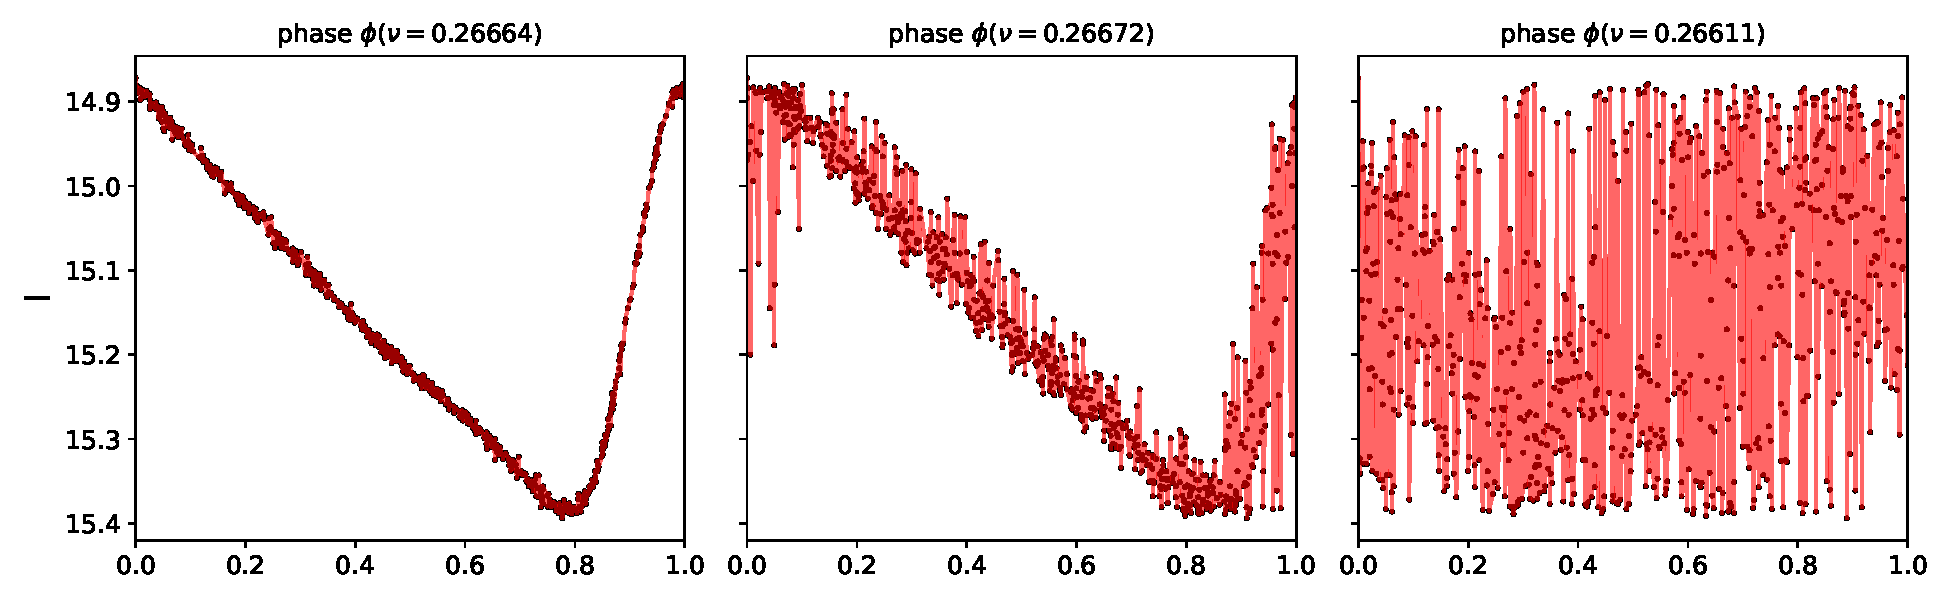
\includegraphics[width=\textwidth]{img/offphase.pdf}
		\caption[Off-frequency phase diagrams: arclength]{
			Different phase diagrams for tests frequencies on the star from figure \ref{fig:mag-phase-2}.
			The red lines are connecting each pair of consecutive dots on the phase diagram,
			and its total length is minimum at the correct phase, and higher otherwise.
			Contrary to \autoref{fig:complex-phase-off}, even the slightest deviation from the correct frequency causes the arclength to rise;
			this method is extremely sensible to phase changes.
		}
		\label{fig:offphase}
	\end{figure}
	
	
	\subsubsection{Phase diagram statistics}
	
	As an alternative to sorting all the phases each time, we could just do it partially,
	dividing the [0,1] phase axis into $M$ equal parts. 
	Then we could use the arclength method with the centroid of the point on those parts, but this does not turn out to be very useful.
	An alternative is the method proposed by \cite{Stellingwerf1978}, which defines the global variance of the phase diagram as
	\begin{equation}
		\sigma^2 = \frac{\sum_k^N (f_k - \bar{f})^2}{N-1}
	\end{equation}
	and a sort of moving variance
	\begin{equation}
		s_j^2 = \frac{\sum_k^{n_j} (f_k-\bar{f}_j)^2}{n_j-1}
	\end{equation}
	where the sum is performed over the $n_j$ points in the $j$-th interval, $j\in[1,M]$.
	The pooled variance for the $M$ samples would be 
	\begin{equation}
		s^2 = \frac{\sum_j^M (n_j-1)s^2}{\sum_j^N n_j -M} \label{eq:pooled-variance}
	\end{equation}
	and the statistic to consider will be defined as $\Theta=s^2/\sigma^2$. 
	If the frequency used to calculate the phases is wrong, $\Theta\approx 1$, and if its right or nearly right, 
	$\Theta$ would reach a local minimum.
	
	This method technically fits the phase curve with the moving mean of the phase curve, and is thus another approximation of the power spectrum.
	The coefficient of determination $R^2=1-\Theta$ could be used directly to compare it with a Lomb-Scargle periodogram, but this method will probably be slower,
	as the tally of a length $n$ array into $M$ sub-intervals is $~O(nM)$.
	
	The same phase diagrams as in \autoref{fig:offphase}, 
	but partially sorted (binned as bidimensional histograms), can be seen in \autoref{fig:offhist2d}.
	Note that this method only requires discretization of the data in the phase axis.
	
	
	\subsubsection{Phase diagram entropy}
	
	If instead of calculating the variance of each column of this histograms,
	we calculate the overall entropy of the data, we would be using the minimum entropy method proposed by \cite{Cincotta1995I}.
	If the phase diagram is partitioned in $m=M^2$ zones of the same area, 
	the probability $\mu_j$ for a point to be inside any given zone is just the points inside that zone divided by the total number of points.
	The entropy of this configuration in the \cite{Shannon1948} sense is 
	\begin{equation}
		S = - \sum_j^m \mu_j \ln(\mu_j) \label{eq:entropy}
	\end{equation}
	As already discussed, if the test period is off, we expect the phase diagram to be populated everywhere; 
	therefore those probabilities would be uniform, and the entropy would be maximum.
	In the correct period the probabilities for each zone are heavily unbalanced towards the occupied spaces,
	and then the histogram is \enquote{ordered} and the information entropy minimum.
	
	On a more mathematical level, if the histogram is populated everywhere, as in the noise case, 
	most of the $\mu_j$ would be nonzero. As probabilities, they lie in the $[0,1]$ interval, 
	making their logarithms negative, adding up to a positive and maximal sum.
	
	On the other side, on the correct period there would be many unoccupied zones (see \autoref{fig:offhist2d}), 
	and therefore most of the $\mu_j$ would be zero. As $\lim_{\mu\to0}\mu \ln \mu = 0$.
	The growth of the other probabilities cannot compensate for this loss, so the sum is minimum.	
	This has been rigorously proved by \cite{Cincotta1999II}.

	As the obvious implementation involve the full bidimensional binning of the phase diagram, 
	this would be $O(nM^2)$, making it technically slower than the other methods.
	There are faster methods to compute the entropy of a signal \citep{Cohen1985}, 
	but for our purposes it is possible to implement an entropy method that is faster that both 
	the $O(n\ln n)$ arclength and the $O(nM)$ method, by transforming the bidimensional histogram into a one dimensional one;
	see \autoref{lst:entropy-flattened} for details.
	
	\begin{figure}
		\centering
		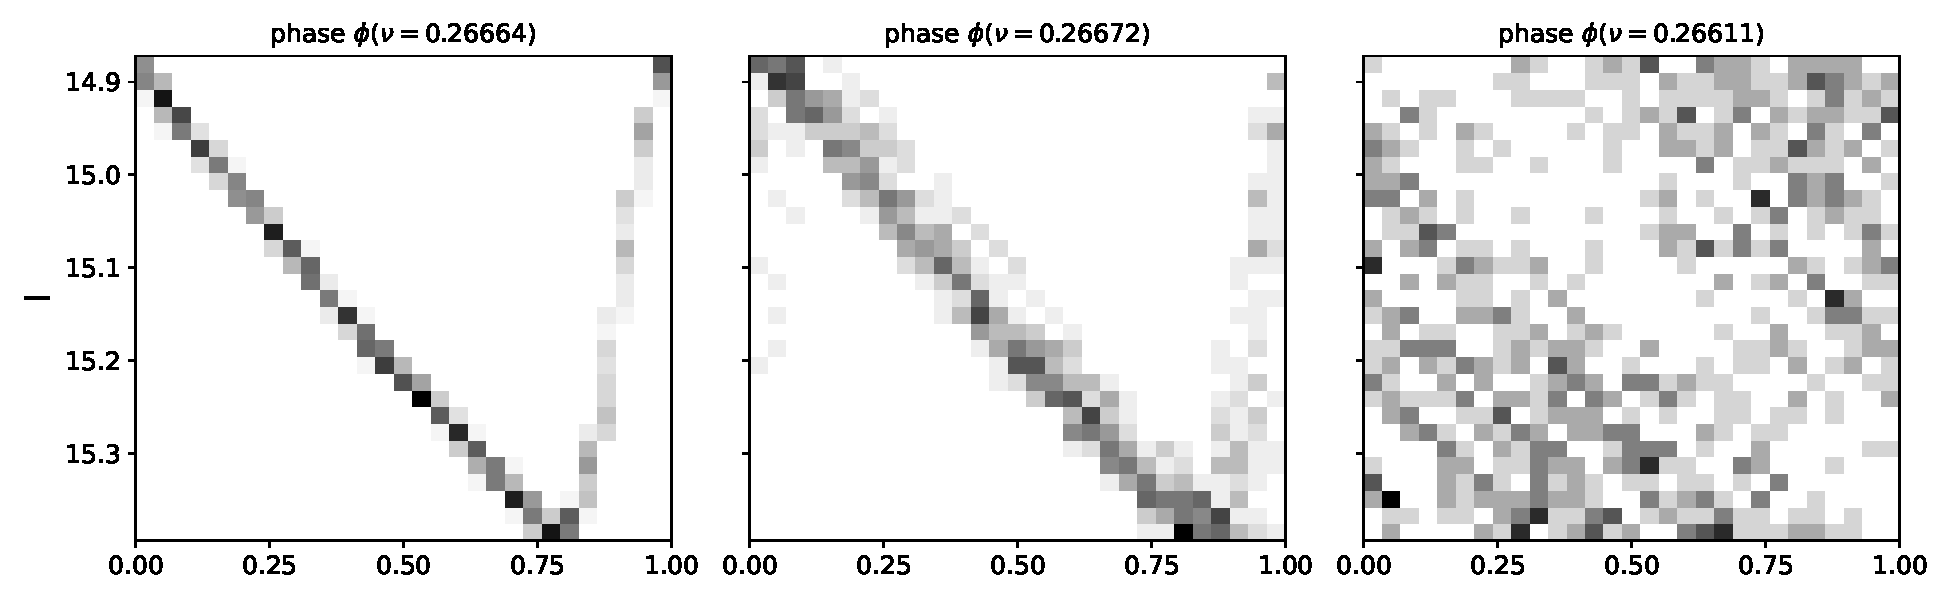
\includegraphics[width=\textwidth]{img/offhist2d.pdf}
		\caption[Off-frequency phase diagrams: histograms]{
			Same as \autoref{fig:offphase} but \enquote{pixelated} phase diagrams, \textit{i.e.} bidimensional histograms.
			$M=30$ bins were taken on each axis, for a total of $m=900$ zones.
			The greater column-wise dispersion of the off-phase diagrams is notable, 
			and when the frequency is completely wrong, the image is just noise.
			On the applications discussed here, the number of bins on each axis are typically between 2 and 10.
		}
		\label{fig:offhist2d}
	\end{figure}




	
	
	
	
	
	
	
	
	
	
	
	
	
	
	
	
	
	
	
	
	
	
	
	
	
	
	
	
	
	
	
	
	
	